%!TEX root = ../../thesis.tex

\section{The diversity of exoplanets}
\label{sec:exoplanet_diversity}
Exoplanetary detections have challenged the theoretical formation models with their variety and distribution of sizes and, locations.
For instance, the discovery of the hot-Jupiter class (large mass planets on close in orbits) challenged the accepted planet formation theories at the time~\citep[.e.g][]{pollack_formation_1996, boss_giant_1997} in which our Solar System was thought to be typical with small rocky planets close to the Sun and large giant planets further away.

The precise characterization of more exoplanets with the detection of exoplanetary atmospheres will allow for the constraints of exoplanetary composition and formation mechanisms to be improved.
For instance, the core accretion model has been able to reproduce the large number of super-Earths, the correlation between star metallicity and planet frequency~\citep[e.g.][]{santos_spectroscopic_2004, fischer_planetmetallicity_2005}, and the presence of many Hot-Jupiter and Neptune like planets in close-in orbits, with the help of migration mechanisms~\citep[e.g.][]{triaud_exoplanets_2016}.
Recent models also combine both planetary formation and evolution to describe the observed exoplanets~\citep[e.g.][]{mordasini_characterization_2012} and can reproduce general population properties in a statistically significant way~\citep{mordasini_extrasolar_2009}.

A proxy for the composition and structure of an exoplanet is the average density, computed from the mass and radius.
A mass-radius diagram is shown in \cref{fig:santerne2018} for Earth-like rocky planets.
The tracks show contours of mass-radius for different theoretical compositions~\citep{brugger_constraints_2017}, while the circles indicate a number of detected small mass exoplanets, with {K2-229\,b} being a super-Earth with a Mercury-like density~\citep{santerne_earthsized_2018}.
The density can give an approximate composition but for a given mass there are an infinite number of combinations of metal/silicate/ice and gas that can produce the same radii~\citep[e.g.][]{seager_massradius_2007}.
Low mass planets tend to be rocky and tend to have small or no atmosphere.
With rock being in-compressible, to first order, it is relatively insensitive to the incident flux.
The radii of solid exoplanets are sensitive to gas content of the atmosphere as a small increase in \ce{H} and/or \ce{He} can cause a large increase in radius~\citep{adams_ocean_2008}.

\begin{figure}
    \centering
    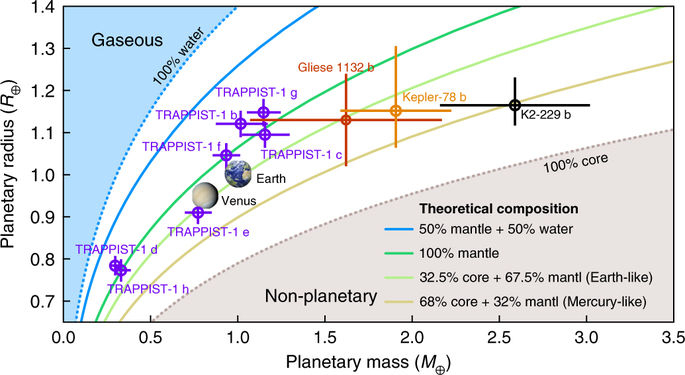
\includegraphics[width=0.7\linewidth]{figures/introduction/santerne_2018}
    \caption[Mass-Radius diagram for rocky planets with composition contours.]{Mass-Radius diagram for rocky planets with composition contours.
        Adapted from~\citet{santerne_earthsized_2018}}
    \label{fig:santerne2018}
\end{figure}

When the gas component becomes dominate, planets begin to have radii independent of their mass~\citep[e.g.][]{lopez_understanding_2014}.
The atmospheres of gas giants are also susceptible to stellar irradiation, with close in Hot-Jupiters having inflated atmospheres and larger radii~\citep[e.g][]{fortney_interior_2010}.
Evaporation has also been used to explain exoplanet properties, such as the Fulton gap. A gap between super-earths and mini-neptunes with radii between 1.5--2.0 \Rearth{}~\citep{fulton_californiakepler_2017}.

\begin{figure}
    \centering
    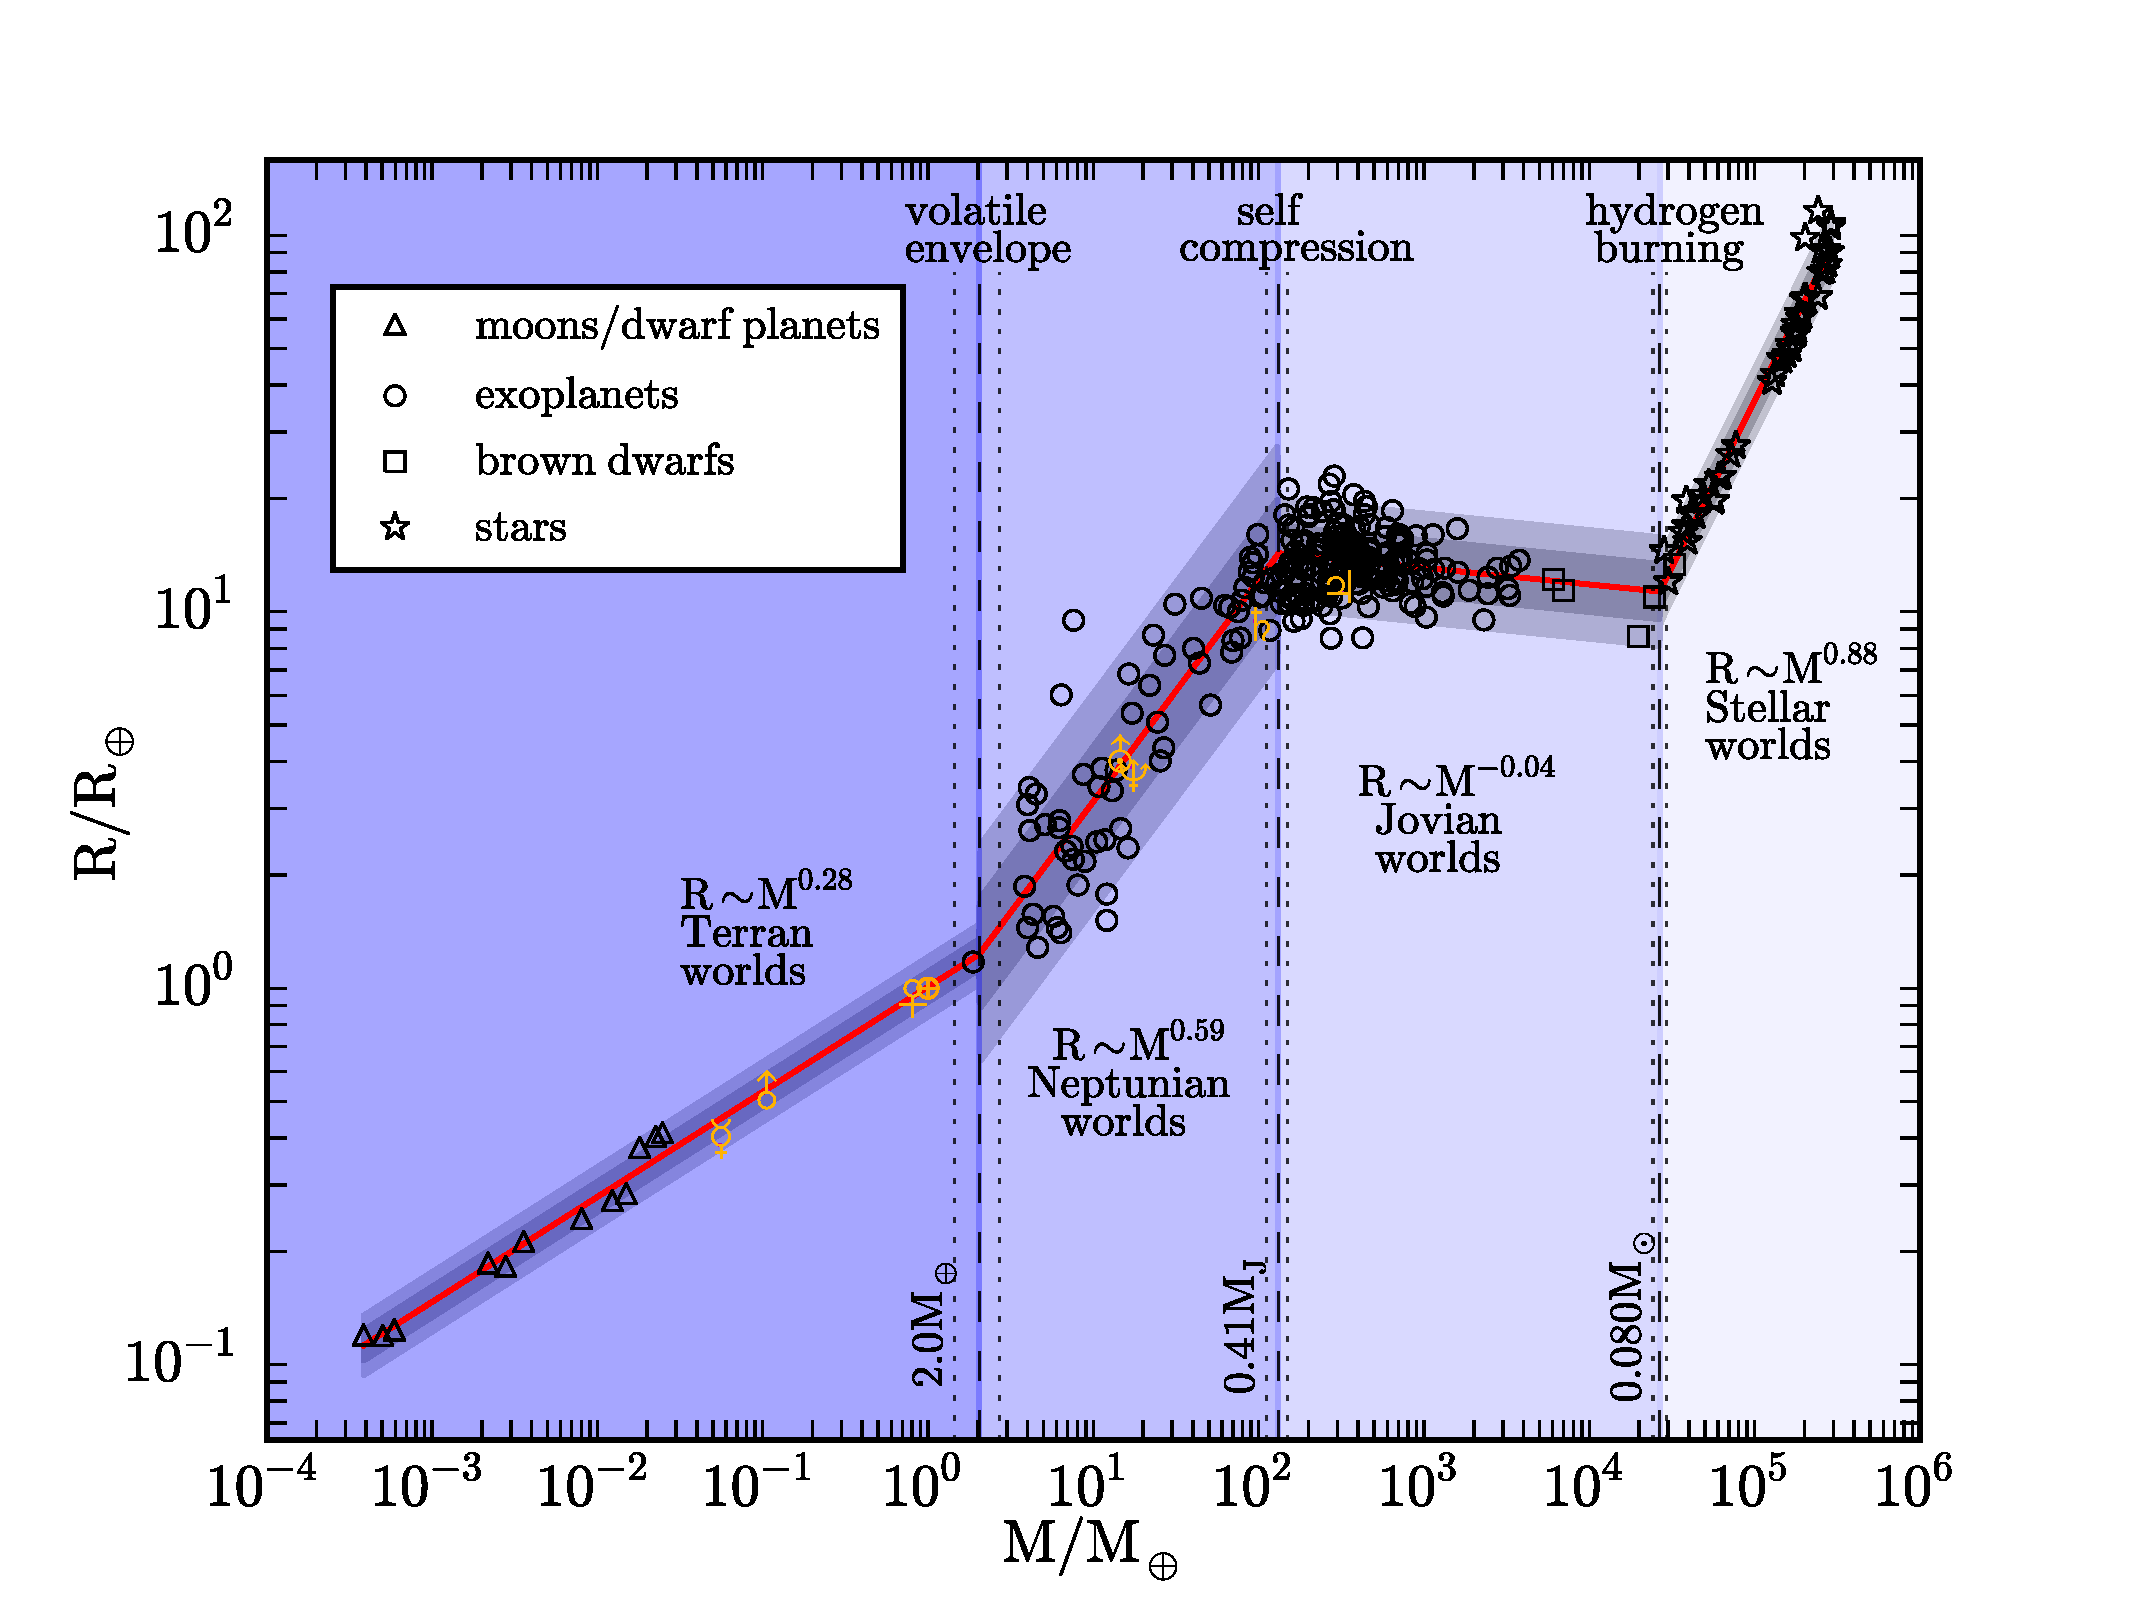
\includegraphics[width=0.7\linewidth]{./figures/introduction/mass_radius_relation.pdf}  \\
    \caption[Mass-Radius relationship with probabilistic fit.]{Mass-Radius relationship with probabilistic fit from dwarf planets to late-type stars from~\citet{chen_probabilistic_2016}.
    The black symbols represents the objects used to fit the model, with the key in the top-left, while the orange symbols represent the solar system planets.
    The red line indicates the average value, while the light and dark grey regions indicate the 65\% and 95\% confidence intervals.}
    \label{fig:mass_radius_relation}
\end{figure}

Models of the mass-radius relation are important as they enable insight into the likely planetary properties when only either mass or radius can or has been measured.
For example~\citet{chen_probabilistic_2016} developed a probabilistic model over 9 orders-of-magnitude in mass and 3 orders-of-magnitude in radius, with the result shown in \cref{fig:mass_radius_relation}.
There are four separate power laws and three different transition regions fitted by the model.
This breaks the mass radius relation into different regions classified after a representative example from our solar system.
The lowest mass range is the rocky "Terran" worlds up to 2.0\,\(\textrm{M}_oplus\) and inclusive of dwarf planets, "Neptunian" worlds between 2.0,\(\textrm{M}_oplus\) and 0.41\,\Mjup{} and, "Jovain" worlds between 0.41\,\Mjup{} and 0.08\Msun{}.
The transitions regions are indicative of a changing composition or physical processes (such as the hydrogen burning limit in stars) and consistent with other works~\citep[e.g.][]{weiss_mass_2013, dieterich_solar_2014, hatzes_definition_2015, rogers_most_2015}.

\subsection{Brown Dwarfs: bridging the gap}
%\todo{I would suggest you make a new section here! Maybe called: Brown-dwarfs: bridging the gap. And this text is perfect for that section. Maybe actually you can add a bit more stuff inside (more details about some of the things you say). This suggestion is to allow the reader to make the bridge between the planets (all you talked up to now) and the brown-dwarfs (that you tried to study in your thesis).}
Recently, there has been a renewed interest in Brown Dwarf (BD) candidates triggered by exoplanetary searches as they bridge the gap between giant planets and low-mass stars.
It is difficult to distinguish between giant planets and {BD}s with a loosely suggested definition of mass between 13--80\,\Mjup{}\footnote{0.01--0.08\Msun{}} for Brown Dwarfs as this is between the Deuterium fusion mass of around 13\,\Mjup{}~\citep[e.g.][]{spiegel_deuteriumburning_2011} and the Hydrogen fusion limit of 80\,\Mjup{}~\citep{chabrier_theory_2000, dieterich_solar_2014}.
Several works found similar properties on the two populations, like a similar density~\citep{hatzes_definition_2015, chen_probabilistic_2016} seen in \cref{fig:mass_radius_relation} by the same power law spanning giant planets and {BD}s, while others have found intriguing differences.
When classified using just mass and size~\citet{chen_probabilistic_2016} find no difference between giant planets and Brown Dwarfs, with Brown Dwarfs just being large giant planets.

There is a paucity of {BD} companions in short period orbits around Sun-like stars (\(\lesssim{}5 \)\AU{}), compared to stellar or planetary companions, termed the \emph{brown dwarf desert}~\citep{halbwachs_exploring_2000, zucker_analysis_2001, sahlmann_search_2011, ranc_moa2007blg197_2015} which can been seen as the gap in the "Jovian" worlds section of \cref{fig:mass_radius_relation}.
There are observed differences in the host star metallicity~\citep{maldonado_searching_2017, santos_observational_2017, schlaufman_evidence_2018} and orbital eccentricity distribution~\citep{ma_statistical_2014} either side of the period/mass gap with the lower mass {BD}s having properties similar to giant planets and high mass {BD}s having properties more like stars.
There is a very strong hint of different formation mechanisms as {BD}s below the gap may primarily form via gravitational instability in protoplanetary disks, while above this gap {BD}s may form more like stellar binary from molecular cloud fragmentation~\citep{ma_statistical_2014}.

As the number of known {BD}s orbiting solar type stars is low, the characterization of benchmark {BD}s in the brown dwarf desert~\citep[e.g.][]{crepp_trends_2016} is beneficial in understanding this sub-stellar population and to help constrain formation and evolution theories~\citep{whitworth_formation_2007}.
There is an inherent degeneracy between the mass, age and luminosity of a given BD~\citep{burrows_nongray_1997} because without sustained fusion, {BD}s cool down over time with an age-dependent cooling rate.

{BD}s in binary systems, unlike free-floating {BD}s~\citep[e.g][]{gagne_simp_2017}, allow for the determination of their masses, when complemented with radial velocity ({RV}) and astrometry measurements.
The {RV} technique provides the mass lower-limit (\Mtwosini{}) of binary and planetary companions, while complementary astrometry measurements can often provide mass upper-limits~\citep[e.g.][]{sahlmann_search_2011}.
Measuring or tightening the constraints of {BD} masses improves the understanding of mass dependence on {BD} formation processes.
Photometry along with stellar evolution models~\citep[e.g.][]{baraffe_evolutionary_2003,allard_btsettl_2013} can also be used to estimate the mass of {BD} companions~\citep[e.g.][]{moutou_eccentricity_2017} if there is sufficient orbital separation, and a precise determination of the age~\citep{soderblom_ages_2010}.


Without sustained fusion, brown dwarfs are relatively cool, and cool down over time, with temperatures below around {3000\K{}} with a few BDs discovered with effective temperatures around 600\K{}\citep{leggett_physical_2009}.
At temperatures below 2600\K{} BD atmospheres become cool enough for condensation and the formation of molecular clouds and hazes~\citep{allard_atmospheres_2012, helling_atmospheres_2014}.
Their spectra are rich with broad molecular bands as well as narrow neutral atomic species.
They are dim and emit a majority of their light at infrared wavelengths, thus can be difficult to detect with optical instrumentation.
However, they are a prime target for \nir{} instrumentation, such as CRIRES \citep[e.g.][]{guenther_prospects_2006,crossfield_global_2014}.


%\begin{figure}[t]
%    \centering
%    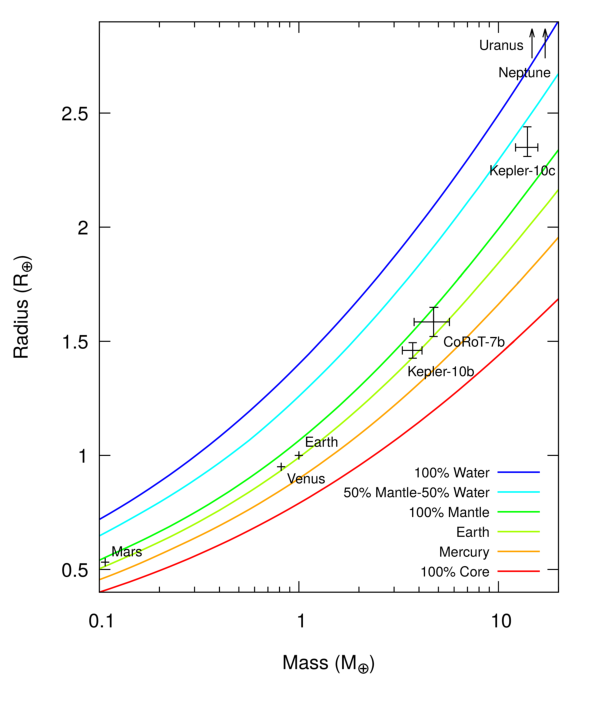
\includegraphics[width=0.4\linewidth]{./figures/introduction/Mass_radius_relation-compostion_Brugger_2017.pdf}
%    \caption[]{Mass-Radius relationship for (super) Earth-like planets with composition contours.
%        Adapted from~\citet{brugger_constraints_2017}}
%    \label{fig:mass_radius_relation_composition}
%\end{figure}
%
%
%
%\begin{figure}
%    \centering
%    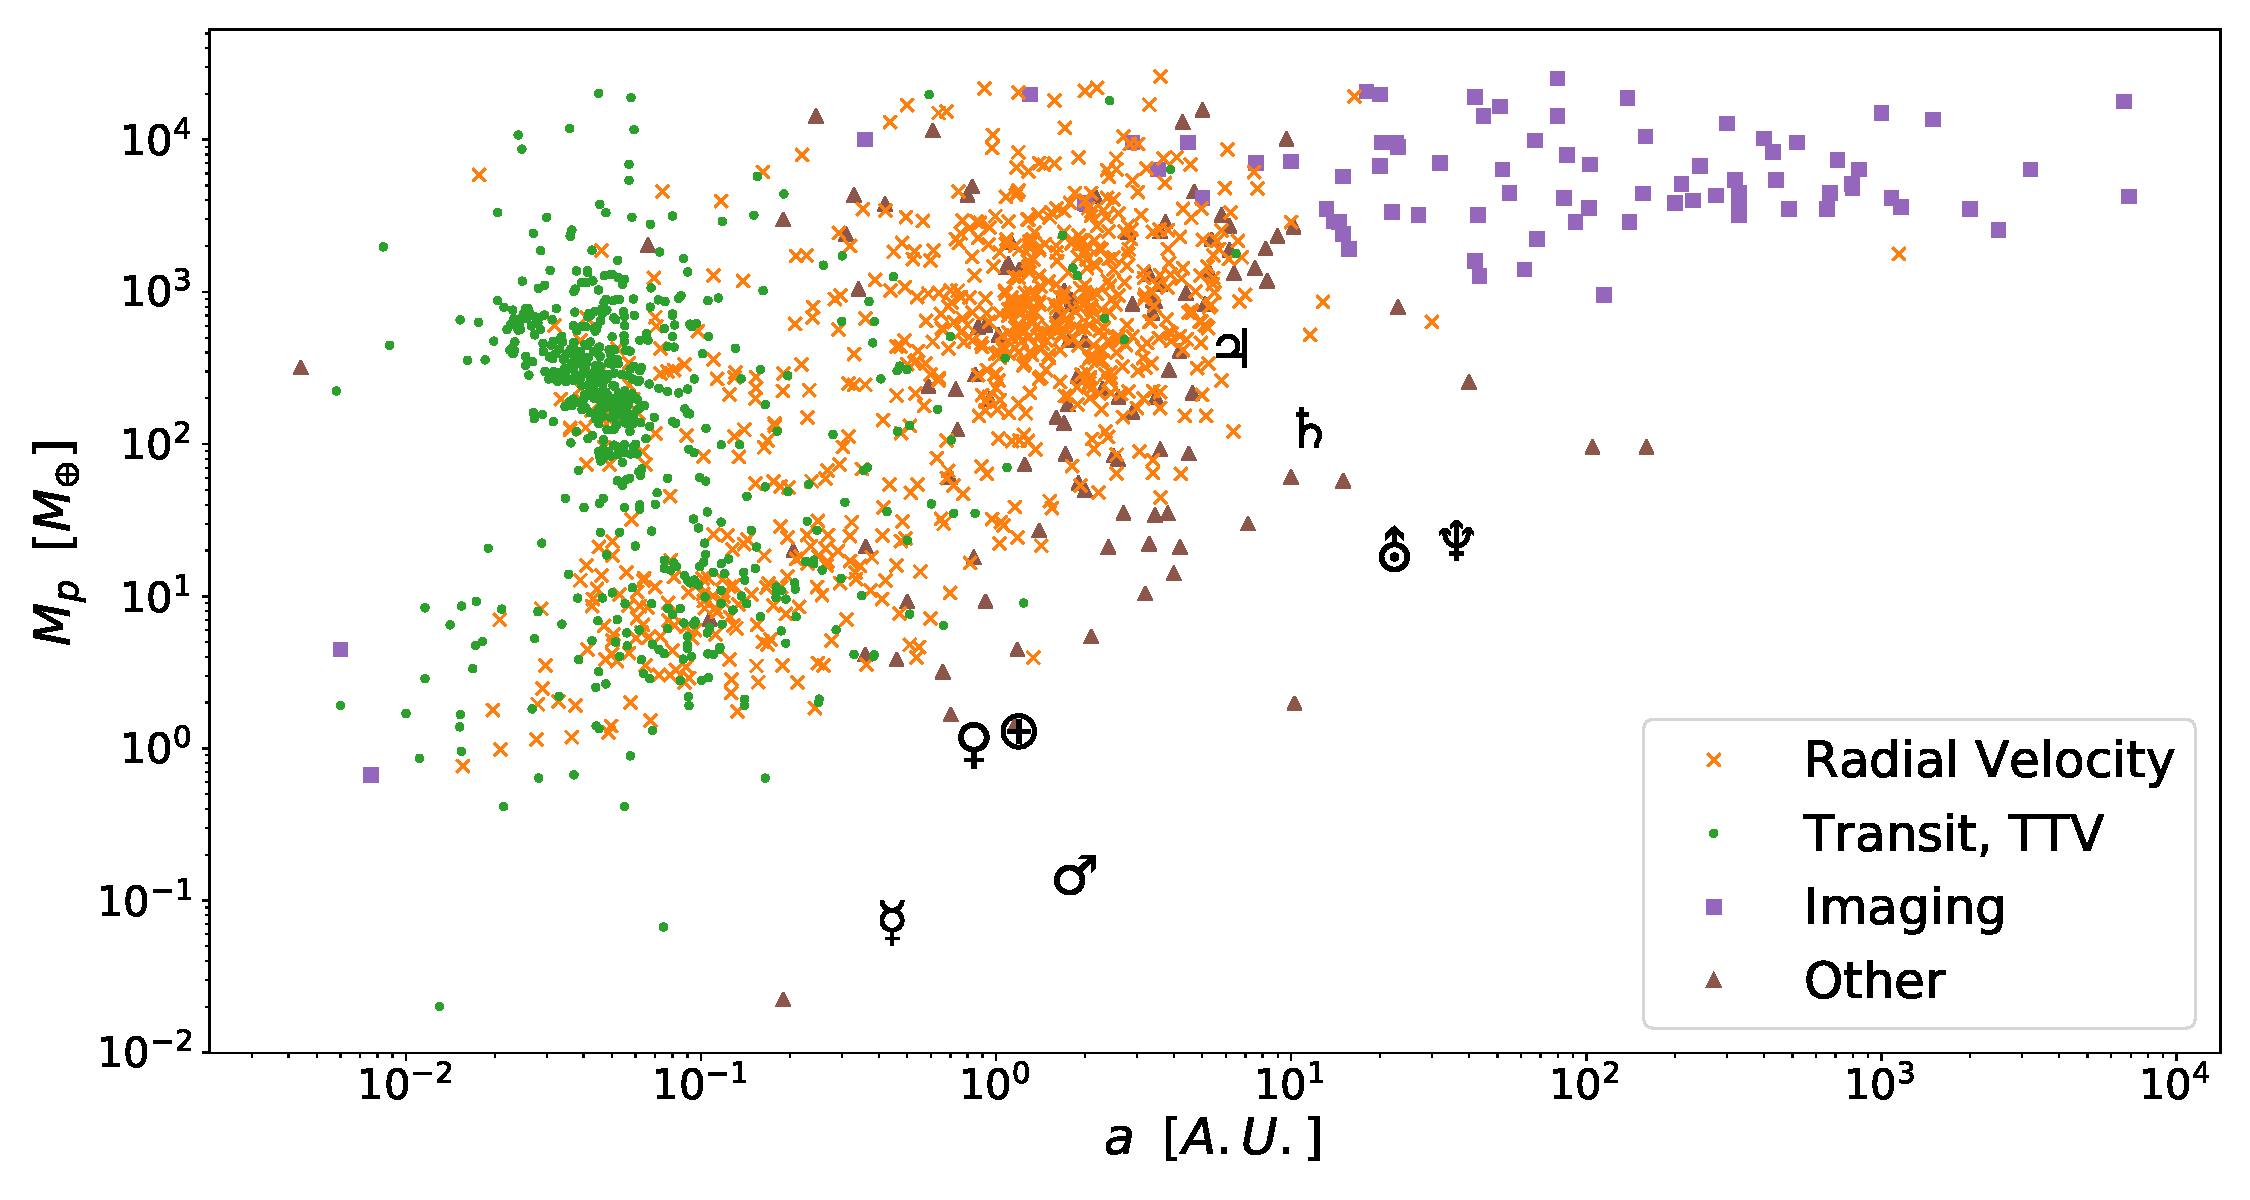
\includegraphics[width=0.\linewidth]{./figures/introduction/exoplanetEU_a_mass.pdf}
%    \caption[]{Exoplanet semi-major axis verses mass diagram.
%        The symbols indicate the location of the solar system planets, $\mercury$-Mercury, $\venus$-Venus, $\earth$-Earth, $\mars$-Mars, $\jupiter$-Jupiter, $\saturn$-Saturn, $\uranus$-Uranus, $\neptune$-Neptune.
%        Data from \href{http://ww.exoplanet.eu}{exoplanet.eu} October 2018}
%    \label{fig:pltoverlayadd}
%\end{figure}
%
%
%Explore what these method have found with exoplanet populations.
